\documentclass[review,preprint]{elsarticle}

%% Use the option review to obtain double line spacing
%% \documentclass[authoryear,preprint,review,12pt]{elsarticle}

%% Use the options 1p,twocolumn; 3p; 3p,twocolumn; 5p; or 5p,twocolumn
%% for a journal layout:
%% \documentclass[final,1p,times]{elsarticle}
%% \documentclass[final,1p,times,twocolumn]{elsarticle}
%% \documentclass[final,3p,times]{elsarticle}
%% \documentclass[final,3p,times,twocolumn]{elsarticle}
%% \documentclass[final,5p,times]{elsarticle}
%% \documentclass[final,5p,times,twocolumn]{elsarticle}

\usepackage{hyperref}
\usepackage{amsmath}
\usepackage{amssymb}
\usepackage{braket}
\usepackage{siunitx}
\usepackage[version=4]{mhchem}
\usepackage{tikz}
\usetikzlibrary{positioning}
\usetikzlibrary {arrows.meta} 
\usepackage{paralist}
\usepackage{todonotes}
\usepackage{tabularray}

\DeclareMathOperator{\erf}{erf}

%% The lineno packages adds line numbers. Start line numbering with
%% \begin{linenumbers}, end it with \end{linenumbers}. Or switch it on
%% for the whole article with \linenumbers.
%\usepackage{lineno}

\journal{Journal of Molecular Liquids}

\begin{document}
	
	\begin{frontmatter}
		
		%% Title, authors and addresses
		
		\title{Solvent effects on the prediction of redox potentials: application to nitroxides}
		
		\author[1]{Pierre Beaujean\corref{cor1}}
		
		\ead{pierre.beaujean@unamur.be}
		
		\cortext[cor1]{Corresponding author}
		
		\affiliation[1]{organization={Theoretical Chemistry Laboratory, Unit of Theoretical and Structural Physical Chemistry, Namur Institute of Structured Matter, University of Namur},%Department and Organization
			addressline={Rue de Bruxelles, 61}, 
			city={Namur},
			postcode={B-5000}, 
			country={Belgium}}
		
		\begin{abstract}
			This paper investigates the impact of solute-solvent effects on the redox potentials of nitroxides, with a focus on ionic interactions caused by the presence of electrolytes found in different environment such as batteries. Indeed the Born model highlights the stabilization of charges due to solvent dielectric constant changes, while solute-ion interactions, influenced by electrolyte presence, play a crucial role. The study reveals that moderate electrolyte concentrations stabilize charged compounds through the Debye-Hückel (DH) effect, and higher concentrations lead to ion-pair formation, both affecting redox properties. The analysis of various nitroxide families shows that ion-substituent interactions, especially in aromatic systems, significantly influence complex stability. In particular, in acetonitrile, the hydroxylamine anion and its cation exhibit strong interactions near the nitroxyl moiety, but only if the nitroxyl is well positioned. The study also confirm that an electrostatic interaction model can predict the effects of substituents, aromaticity, and ring size on redox potentials of nitroxides. 
		\end{abstract}
		
		
		%%Graphical abstract
		\begin{graphicalabstract}
			%\includegraphics{grabs}
		\end{graphicalabstract}
		
		%%Research highlights
		\begin{highlights}
			\item Research highlight 1
			\item Research highlight 2
		\end{highlights}
		
		\begin{keyword}
			%% keywords here, in the form: keyword \sep keyword
			Nitroxide 
			\sep Electrolyte 
			\sep Redox potential
			\sep Debye-Hückel 
			\sep Ion pairs 
			\sep Quantum chemistry
			
			%% PACS codes here, in the form: \PACS code \sep code
			
			%% MSC codes here, in the form: \MSC code \sep code
			%% or \MSC[2008] code \sep code (2000 is the default)
			
		\end{keyword}
		
	\end{frontmatter}
	
	% \linenumbers
	
%% main text
\section{Introduction}


The quest for efficient and sustainable energy storage solutions has intensified research into various battery chemistries. Among these, nitroxide-based batteries have attracted, since their first application in 2002 \cite{nakaharaRechargeableBatteriesOrganic2002}, significant attention due to their high theoretical capacity \cite{friebeSustainableEnergyStorage2019,ernouldNitroxidesBatteryrelatedApplications2021,keDesigningStrategiesAdvanced2023}. They are generally used, like other radical polymers, as cathode materials \cite{okaRadicalPolymersRechargeable2020a,assummaNewConductingCopolymer2020}. Beyond their application in batteries, nitroxides have been extensively studied and utilized in various fields. They serve as spin labels in electron paramagnetic resonance spectroscopy \cite{torricellaNitroxideSpinLabels2021}, as mediators for organic radical reactions and polymerizations \cite{tebbenNitroxidesApplicationsSynthesis2011,leifertOrganicSynthesisUsing2023}, in organic electronic devices \cite{jiAirStableOrganicRadicals2020,xieNitroxideRadicalPolymers2021}, and as antioxidants in biological systems  \cite{souleChemistryBiologyNitroxide2007,lewandowskiNitroxidesAntioxidantsAnticancer2017,prescottBiologicalRelevanceFree2017}.

Nitroxides are organic compounds containing the nitroxyl/aminoxyl radical functional group \cite{berlinerHistoryUseNitroxides2012}. This group can exist in three redox states: the nitroxide radical ($>$\ce{N-O^.}, also shortened as \ce{N^.} in this article), which can be oxidized to the oxoammonium cation ($>$\ce{N+=O}, abbreviated \ce{N+}) or reduced to the hydroxylamine anion ($>$\ce{N-O-}, abbreviated \ce{N-}), as depicted in Fig.~\ref{fig:states}. The remarkable stability of the nitroxide radical arises from the delocalization of the unpaired electron over the nitrogen and oxygen atoms, combined with the steric protection provided by the substituents, and environmental effects due to the interaction with solvent and ions \cite{grynovaOriginScopeLongRange2013,grynovaSwitchingRadicalStability2013}. 

\begin{figure}[!h]
	\centering
	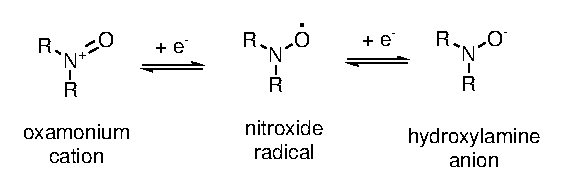
\includegraphics[width=.7\linewidth]{Figure1}
	\caption{Oxidized (left) and reduced (right) forms of the the nitroxide radical (center).}
	\label{fig:states}
\end{figure}

Experimental studies have demonstrated that the performance of nitroxide-based batteries is influenced by substituents \cite{sugaCathodeAnodeActivePoly2007}, solvation, and the nature of the electrolytes used \cite{armandIonicliquidMaterialsElectrochemical2009,strehmelRadicalsIonicLiquids2012,wylieIncreasedStabilityNitroxide2019b}. Understanding the interplay between the nitroxides, the solvents, and the electrolytes is therefore crucial for the rational design of high-performance batteries. Computational studies using quantum chemical methods provide valuable insights into the crucial solvation effects, enabling the prediction and tuning of redox properties.

From a phenomenological perspective, two approaches can be used: at low concentrations in electrolytes, the Debye-Hückel (DH) theory \cite{kontogeorgisDebyeHuckelTheoryIts2018,silvaDerivationsDebyeHuckel2022,silvaImprovingBornEquation2024} provides an initial estimate for interactions within an ionic liquid. While improvements have been proposed over the years to better account for ion-solvent interactions, particularly by including dipole-ion \cite{silvaImprovingBornEquation2024} and quadrupole-ion interactions \cite{slavchovQuadrupoleTermsMaxwell2014,slavchovQuadrupoleTermsMaxwell2014a,coxQuadrupolemediatedDielectricResponse2021}, there have been only a few attempts \cite{matsuiDensityFunctionalTheory2013,xiaoReorganizationEnergyElectron2013,xiaoMolecularDebyeHuckelApproach2014} to incorporate DH theory into the prediction of redox potentials. There is also a limited implementation of DH theory in the polarizable continuum model \cite{cossiInitioStudyIonic1998}. 

At high concentrations (such as in ionic liquids), ion-pair formation can be expected \cite{marcusIonPairing2006}. Alongside electrostatic models \cite{krishtalikElectrostaticIonSolvent1991,lundDielectricInterpretationSpecificity2010}, various theoretical calculations of redox potentials have been performed \cite{mehtaTheoreticalInvestigationRedox2007,quAccurateModelingEffect2016,taherkhaniInvestigationIonPairs2022}, indicating that such interactions can be significant. This has also been recently investigated experimentally by Mugisa et al. \cite{mugisaEffectIonparingKinetics2024}, who assessed the impact of complexation on the thermodynamic and kinetics of  the reduction  of charged metal complexes.

Therefore, while seminal studies by Coote and co-workers \cite{hodgsonOneElectronOxidationReduction2007,blincoExperimentalTheoreticalStudies2008} have focused on the impact of substituents on the redox potential of nitroxides, later investigations by other groups have also considered the effect of the nature of the electrolytes and of the various nitroxide-electrolyte interactions between them, including electrostatic interactions. For example, in 2019, Wylie and co-workers \cite{wylieImprovedPerformanceAllOrganic2019a,wylieIncreasedStabilityNitroxide2019b} demonstrated that the interactions between the ionic liquid and the nitroxide can increase the redox potential by more than \SI{3}{\volt} for a well-chosen pair of electrolytes. Prior to this, Zhang \textit{et al.} focused on stabilizing the radical-ion interactions \cite{zhangInteractionsImidazoliumBasedIonic2016,zhangEffectHeteroatomFunctionality2018}, showing that the interactions between a cation and the nitroxyl group are driven by both electrostatic and dispersion effects.

In this study, the impact of solvation at low and high concentrations in electrolytes is investigated by using theoretical chemistry methods on the redox potential of various nitroxides. Since the impact of different electrolytes has already been addressed, the focus is on the effects of the skeleton bearing the nitroxyl group, categorized into five families (Fig.~\ref{fig:families}), and of the substituents. To facilitate comparison with experimental data, two solvents are considered: water and acetonitrile, for which experimental results are available \cite{morrisChemicalElectrochemicalReduction1991,goldsteinStructureActivityRelationship2006,blincoExperimentalTheoreticalStudies2008,zhangEffectHeteroatomFunctionality2018}. 
Different (semi-)quantitative models are employed at each step to aid in the interpretation of the results. It should be noted that the reduced form (hydroxylamine anion) is generally not found in solution \cite{israeliKineticsMechanismComproportionation2005}, as further proton additions (depending on the pH) are involved to form the hydroxylamine or the hydroxylamonium cation. These species were not considered in this article, and thus only experimental oxidation potentials (first reaction in  Fig.~\ref{fig:states}) are compared to the theoretical predictions.

This paper is organized as follows: Section \ref{sec:theory} introduces key concepts and models. The methodology used in this study is detailed in Section \ref{sec:methodo}. The results are then presented in four parts: the impact of substituents on the redox properties is discussed in Section \ref{sec:sar}, followed by an analysis of the effects of solvents in Section \ref{sec:solv}, and the influence of electrolytes in Section \ref{sec:elect}. Finally, a comparison between theoretical predictions and experimental results is provided in Section \ref{sec:exp}. Conclusions and future outlooks are presented in Section \ref{sec:conclusion}.

\begin{figure}[!h]
	\centering
	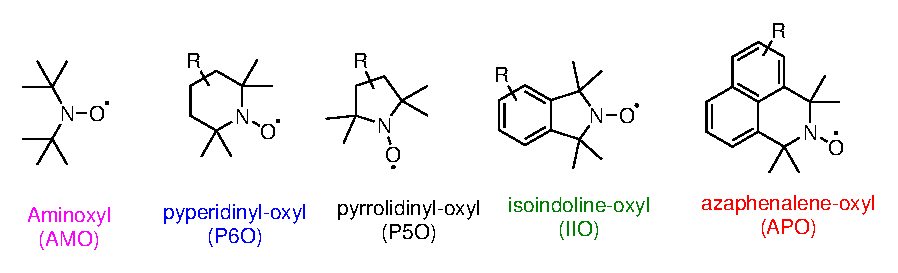
\includegraphics[width=\linewidth]{Figure2}
	\caption{Families of nitroxide compounds.}
	\label{fig:families}
\end{figure}

\section{Theory}\label{sec:theory}

\subsection{Redox potentials in solution}

According to Ref.~\cite{marenichComputationalElectrochemistryPrediction2014}, the absolute reduction potential $E_{abs}^0$ (in \si{\volt}) of the half-reaction of reduction of $X^z$, $X^{z} + n_e\,e^- \rightarrow X^{z-n_e}$, reads: \begin{equation}
	E_{abs}^0(X^{z}|X^{z-n_e}) = -\frac{\Delta G_{r}^\star}{n_e\,F}, \text{ with } \Delta G_{r}^\star = G^\star(X^{z-n_e}) - G^\star(X^z), \label{eq:nernst}
\end{equation}
where $\Delta G_{r}^\star$ is the Gibbs free energy of the reduction reaction in solution, $F$ is the Faraday constant (\SI{9.648533e4}{\coulomb\per\mole}) and $n_e$ the number of electrons involved in the reduction process. Moreover, $G^\star(X^z)$ is the Gibbs free energy of $X^z$ in solution.  In the rest of this article, it is considered that $G^\star(e^-) = 0$.

While there is some validity in using the adiabatic ionization/electron affinity potentials instead of the full Gibbs free energy change when the reorganization energy (in the sense of Marcus theory, referring to the geometry relaxation between two redox states) is small, allowing for precise the use of post-Hartree Fock methods  \cite{namazianBenchmarkCalculationsAbsolute2010,marenichComputationalElectrochemistryPrediction2014,makosModelingAbsoluteRedox2022}, this condition is not met in the present study, which would require to evaluate geometry reorganization and solvent effects at a different level. Consequently, a coherent treatment at the DFT level is chosen for this article.


The comparison between relative (vs SHE) experimental and calculated reduction potential is performed using a common reference:\begin{equation}
	E^0_{rel}(X^z|X^{z-n_e})  = E^0_{abs}(X^z|X^{z-n_e}) - E^{0}_{abs}(\text{SHE}), \label{eq:ecalc}
\end{equation}
with $E^0_{abs}(\text{SHE}) = \SI{4.28}{\volt}$ in water or \SI{4.52}{\volt} in acetonitrile \cite{marenichComputationalElectrochemistryPrediction2014}.


\subsection{Debye-Hückel theory}

From a phenomenological perspective, such $G^\star(X^z)$ values are the sum of the system's energy in vacuum, $G^0(X^z)$, and the change in (free) energy resulting from its transfer to an electrolytic solution, $\Delta G_S^\star(X^z)$. Using the thermodynamic cycle presented in Figure \ref{fig:th}, the latter can be further decomposed int four steps: $\Delta G_d + \Delta G_s$ (``d" means the discharge of in the gas phase followed by,  ``c'' charge in a dielectric) accounts for purely electrostatic processes, while $\Delta G_s$ is primarily due to non-electrostatic contributions (cavitation, van der Waals forces, etc.). Finally, $\Delta G^\star_{DH}$ incorporates the effect of the` surrounding ions and is therefore crucial when dealing with electrolytes \cite{silvaImprovingBornEquation2024}.


\begin{figure}[!h]
	\centering
	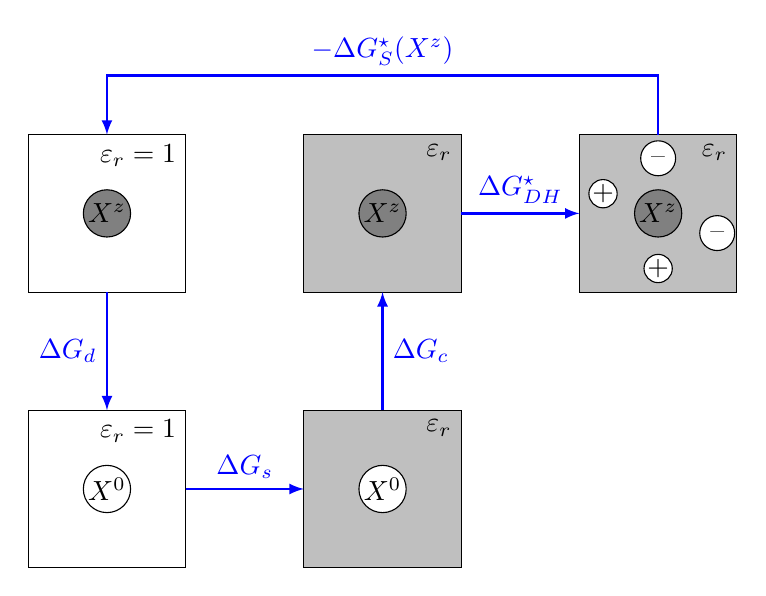
\begin{tikzpicture}
		\draw (-1,-1) rectangle +(2,2) node[anchor=north east]{$\varepsilon_r=1$};
		\draw[fill=gray] (0,0) circle (.3cm) node{$X^z$};
		
		
		\draw (-1,-4.5) rectangle +(2,2) node[anchor=north east]{$\varepsilon_r=1$};
		\draw (0,-3.5) circle (.3cm) node{$X^0$};
		
		
		\draw[fill=gray!50] (2.5,-4.5) rectangle +(2,2) node[anchor=north east]{$\varepsilon_r$};
		\draw[fill=white] (3.5,-3.5) circle (.3cm) node{$X^0$};
		
		
		\draw[fill=gray!50] (2.5,-1) rectangle +(2,2) node[anchor=north east]{$\varepsilon_r$};
		\draw[fill=gray] (3.5,0) circle (.3cm) node{$X^z$};
		
		
		\draw[fill=gray!50] (6,-1) rectangle +(2,2) node[anchor=north east]{$\varepsilon_r$};
		\draw[fill=gray] (7,0) circle (.3cm) node{$X^z$};
		\draw (2.8+3.5,-3.25+3.5) node[draw,fill=white,circle,inner sep=0]{+}
		(3.5+3.5,-2.8+3.5) node[draw,fill=white,circle,inner sep=.075cm]{--}
		(4.25+3.5,-3.75+3.5) node[draw,fill=white,circle,inner sep=.075cm]{--}
		(3.5+3.5,-4.2+3.5) node[draw,fill=white,circle,inner sep=0]{+};
		
		\draw[blue,thick,-latex] (0,-1) -- +(0,-1.5) node[midway,left]{$\Delta G_d$};
		\draw[blue,thick,-latex] (1,-3.5) -- +(1.5,0) node[midway,above]{$\Delta G_s$};
		\draw[blue,thick,-latex] (3.5,-2.5) -- +(0,1.5) node[midway,right]{$\Delta G_c$};
		\draw[blue,thick,-latex] (4.5,0) -- +(1.5,0) node[midway,above]{$\Delta G^\star_{DH}$};
		\draw[blue,thick,-latex] (7,1) -- ++(0,.75) -- node[midway,above]{$-\Delta G_S^\star(X^z)$} ++(-7,0) -- ++(0,-.75);
	\end{tikzpicture}
	\caption{Thermodynamic cycle to compute the energy of solvation of an ion, $X^z$, in a electrolyte (solvent characterized by a $\varepsilon = \varepsilon_0\,\varepsilon_r$ dielectric constant and by a ``cloud'' of other ions). $\Delta G_d$ is the Gibbs free energy change associated with the discharge of $X^z$ in gas phase, $\Delta G_s$ is the Gibbs free energy change of the solvation of $X$, $\Delta G_c$ is the Gibbs free energy change associated to the charging of $X$ in $\varepsilon$, and $\Delta G^\star_{DH}$ is the Gibbs free energy change due to the addition of the other ions.}
	\label{fig:th}
\end{figure}


On the one hand, at the quantum chemistry (QC) level, the solvation energy is generally treated implicitly, thanks to a self-consistent reaction field approach (SCRF) \cite{herbertDielectricContinuumMethods2021}, leading to $G^\star_{SCRF}$: \begin{align}
	G^\star_{SCRF}(X) &= \Braket{\Psi(X)|{\hat{H}+\frac{1}{2}\hat{R}}|\Psi(X)} + G_{thermo}[\Psi(X)] + G_{nonelst}(X) \nonumber\\
	&= E[\Psi(X)] + G_{thermo}[\Psi(X)] + \underbrace{G_{elst}[\Psi(X)] + G_{nonelst}(X)}_{\Delta G^\star_{S,SCRF}(X)}, \label{eq:scrf}
\end{align}
where $\Psi$ is the wavefunction of $X$ (minimized under the application of $\hat R$, so not equal to the gas phase wavefunction), $\hat H$ is the electronic Hamiltonian, leading to the electronic energy, $E[\Psi(x)]$, $\hat R$ is the reaction field operator (generally recognized to give rise to the electrostatic contribution to the solvation energy, $G_{elst}$), $G_{thermo}$ are the thermal contributions to the Gibbs free energy derived from thermostatistic analysis, and $G_{nonelst}$ collects the non-electrostatic contributions (cavitation, dispersion, etc) to the solvation energy. Therefore, using the notation of Figure \ref{fig:th} (and assuming no change in the geometry of $X^z$), $ \Delta G^\star_{S,SCRF}(X^z) = \Delta G_d + \Delta G_s + \Delta G_{c}$. $ \Delta G^\star_{S,SCRF}(X^z)$ is, therefore, an approximation to $\Delta G^\star_S(X^z)$, since $\Delta G^\star_{DH}$ is missing. 

On the other hand, the Debye-Hückel (DH) theory provides another estimate of $\Delta G_{S}^\star$ \cite{bockrisModernElectrochemistryIonics1998}. Indeed, assuming that a ion $X^z$, bearing a charge $q = z\,e$ ($e$ is the elementary charge), can be approximated by a sphere of radius $a$ and that the ions in the solution are distributed in the solution according to Maxwell-Boltzmann statistics, one obtains the corresponding solvation energy as \cite{kontogeorgisDebyeHuckelTheoryIts2018,silvaTrueHuckelEquation2022,silvaImprovingBornEquation2024}:\begin{align}
	\Delta G^\star_{S,DH}(X^z)
	&= \Delta G^\star_{Born}(X^z) + \Delta G^\star_{DH}(X^z)\label{eq:adh}
\end{align}
where:
\begin{align}
	&\Delta G^\star_{DH}(X^z) = -\frac{q^2}{4\pi\varepsilon_0\varepsilon_r}\,\frac{\kappa}{(\kappa\,a)^3}\,\left[\ln(1+\kappa\,a)-\kappa\,a+\frac{1}{2}(\kappa\,a)^2\right],\label{eq:dh} \end{align}
in which $\kappa$ is the inverse of the Debye screening length, defined from:\begin{equation}
	\kappa^2 = \sum_i^{\text{electrolytes}} \frac{n_i\,q_i^2}{\varepsilon_0\varepsilon_r\,k_B\,T}, \label{eq:kappa2}
\end{equation}
where $n_i$ is the number density of ion of type $i$ ($n_i = N_i / V = c_i\,\mathcal{N}_a$ where $\mathcal{N}_a$ is the Avogadro number and $c_i$ is the concentration in ion $i$), $k_B$ is the Boltzmann constant (\SI{1.380649e-23}{\joule\per\kelvin}), and $T$ is the temperature (assumed to be \SI{298.15}{\kelvin}).  $\kappa$ is  proportional to the ionic strength of the solution, $I = \frac{1}{2}\sum_i c_i\,z_i^2$. 
Furthermore:
\begin{equation}
	\Delta G^\star_{Born}(X^z) =\frac{q^2}{8\pi\varepsilon_0\,a}\,\left[\frac{1}{\varepsilon_r}-1\right], \label{eq:born}\\
\end{equation}
 The Born part [Eq.~\eqref{eq:born}] is generally dominant in solvation energies predicted by this model (Fig.~S1).
 
 While the SCRF approach neglect $\Delta G^\star_{DH}$, the DH approach approximate $\Delta G_{d}$ and $\Delta G_{c}$ (with the Born model) and neglect $\Delta G_{s}$. Therefore, by combining Eqs.~\eqref{eq:scrf} and \eqref{eq:adh}, one defines:\begin{equation}
	G^\star(X^z) = G^\star_{SCRF}(X^z) + \Delta G^\star_{DH}(X^z), \label{eq:gtot}
\end{equation}
to be used in Eq.~\eqref{eq:nernst}.

\subsection{Modeling the effect of the substituents on the nitroxides and its reduction potential}\label{sec:eleczhang}

The effect of the substituent(s) on the nitroxide can be described using an electrostatic model. Within this model, the interaction occurs between the dipole moment of the non-charged substituent and the charge of the nitroxide (when oxidized or reduced).  Specifically, the charge-dipole interactions stabilize the oxoammonium ($>$\ce{N+=O}) if the dipole is aligned with the charge, while they destabilize the hydroxylamine ($>$\ce{N-O-}), both resulting in a decrease in the redox potential (see Fig.~\ref{fig:dipole}). Within this framework, it is therefore expected that compounds with donor substituents have lower redox potentials than acceptor substituents.


\begin{figure}[!h]
	\centering
	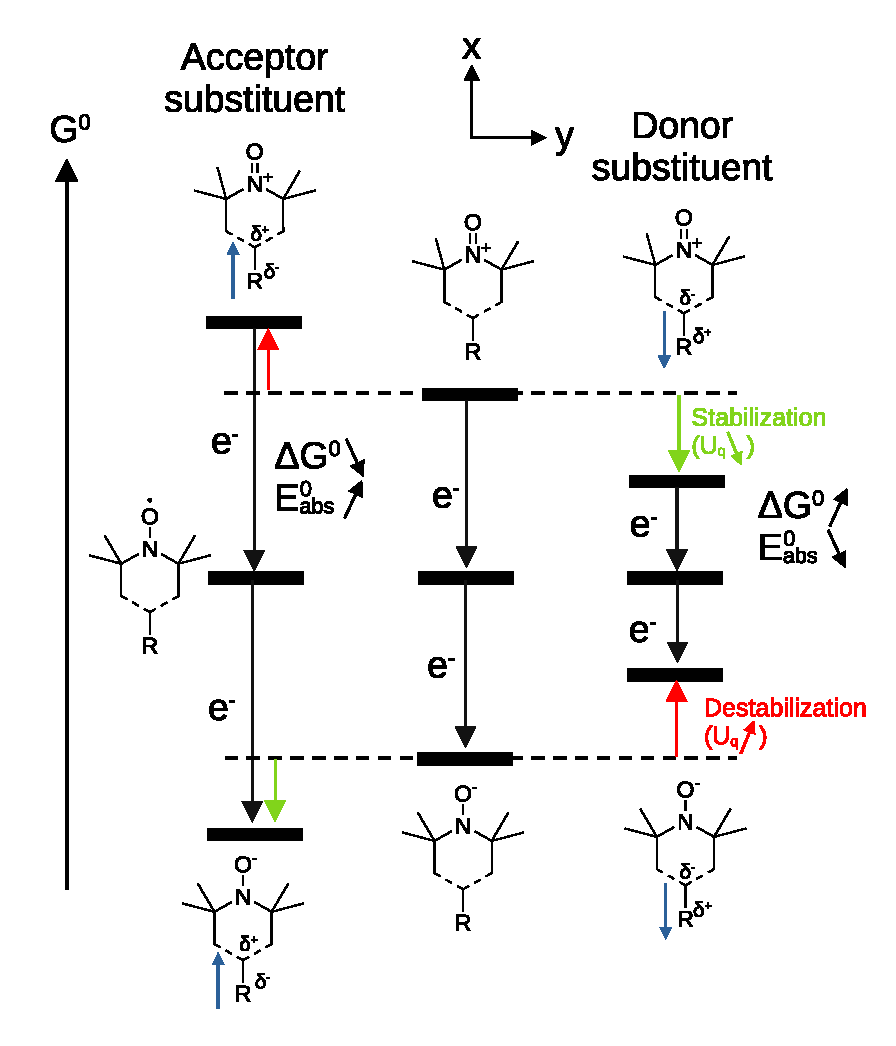
\includegraphics[width=.8\linewidth]{Figure4}
	\caption{Impact of the dipole orientation of the \ce{R} substituent on the redox potential when the dipole is oriented in  the positive $x$ direction (acceptor substituent, left) or not (donor substituent, right).}
	\label{fig:dipole}
\end{figure}

In 2018, building upon previous work by Gryn'ova and co-workers \cite{grynovaOriginScopeLongRange2013,grynovaSwitchingRadicalStability2013}, Zhang \textit{et al.} extended and applied this model to the oxidation potential of nitroxides \cite{zhangEffectHeteroatomFunctionality2018}. They further expanded the electrostatic interaction as multipoles, truncated after the third order, to incorporate the large quadrupole moment of aromatic compounds:
\begin{equation}
	U_q(r) =\frac{1}{4\pi\varepsilon_0} \left[\frac{\mu_x}{r^2} + \frac{Q_{xx}}{r^3}\right], \label{eq:Er}
\end{equation}
assuming a non-charged substituent. The different quantities (dipole moment, $\mu_x$, and traceless quadrupole moment, $Q_{xx}$) are evaluated through a single-point calculation on a simplified structure, using the geometry of the radical where the \ce{N-O^.} moiety is substituted by \ce{CH2}. Since the alignment of the dipole with the charge needs to be accounted for, this geometry is oriented such that the $x$-axis passes through the the carbon bearing the substituent (set as the origin) and the nitrogen. This definition differs from the original model, as Zhang and co-workers \cite{zhangEffectHeteroatomFunctionality2018} did not consider multiple positions for a given substituent. They also only focused on the oxidation, while both redox processes are considered here.


\subsection{Impact of ion-pair formation on redox potentials}

At high concentrations of electrolytes, the formation of ion pairs in solution is expected (further insights are provided in the subsequent subsection). In this study, the electrolyte consists of a pair, \ce{AC}, of counterions, where \ce{A-} and \ce{C+} represent the anion and cation, respectively. Furthermore, two possibilities of complexation are considered: \begin{inparaenum}[(i)]
	\item the pairs \ce{N+A-}, \ce{N^.C+}, and \ce{N^-C+} between the oxidized, neutral and reduced states of the nitroxide  (with a complexation equilibrium constant $K_{x1}$, $x=0$, 1, and 2 for oxidized, radical, and reduced states, respectively), with their corresponding counterions (\ce{A-} and \ce{C+}, respectively), and then
	\item complexation with the \ce{AC} pair (with an equilibrium constant $K_{x2}$), which occurs when the concentration of electrolyte becomes large \cite{wylieImprovedPerformanceAllOrganic2019a}.
\end{inparaenum}
The various equilibrium constants are defined in Fig.~\ref{fig:cip}. Note that only the complexation between the radical species and the cation is considered here, according to previous investigations by Zhang \textit{et al.} \cite{zhangInteractionsImidazoliumBasedIonic2016,zhangEffectHeteroatomFunctionality2018}.


\begin{figure}[!h]
	\centering
	\newcommand{\arrwy}[3]{
		\draw [transform canvas={yshift=0.3ex},arrows = {-Stealth[harpoon]}] (#1) -- (#2) node[midway,above]{#3};
		\draw [transform canvas={yshift=-0.3ex},arrows = {-Stealth[harpoon]}] (#2) -- (#1);
		}
		\newcommand{\arrwx}[3]{
		\draw [transform canvas={xshift=0.3ex},arrows = {-Stealth[harpoon]}] (#1) -- (#2) node[midway,left]{#3};
		\draw [transform canvas={xshift=-0.3ex},arrows = {-Stealth[harpoon]}] (#2) -- (#1);
		}
	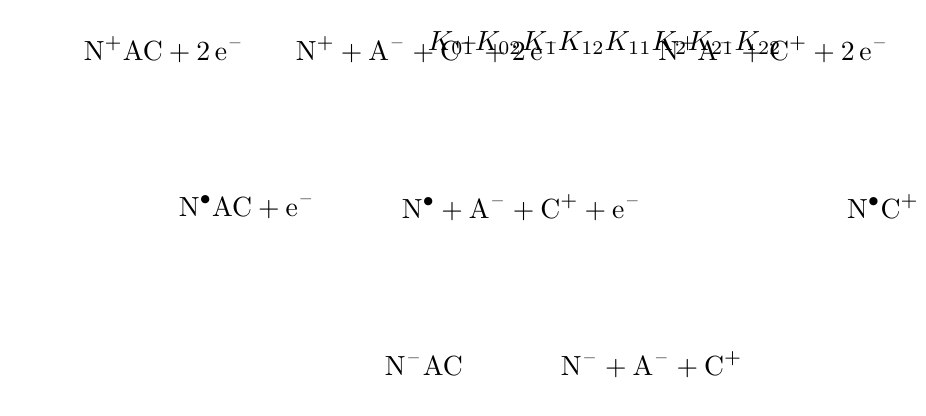
\begin{tikzpicture}[node distance=2cm]
		\node (N1) {\ce{N+ + A- + C+ + 2e-}};
		\node[right=1cm of N1] (N1c) {\ce{N+A^- + C+ + 2e-}};
		\arrwy{N1.east}{N1c.west}{$K_{01}$}
		\node[left=1cm of N1] (N1cc) {\ce{N+AC + 2e-}};
		\arrwy{N1cc.east}{N1.west}{$K_{02}$}
		
		\node[below of = N1] (N2) {\ce{N^. + A- + C+ + e-}};
		\arrwx{N1.south}{N2.north}{$K_{1}$}
		\node[below of=N1cc] (N2cc) {\ce{N^.AC + e-}};
		\arrwy{N2cc.east}{N2.west}{$K_{12}$}
		\node[below of=N1c] (N2c) {\ce{N^.C+ + A- + e-}};
		\arrwy{N2.east}{N2c.west}{$K_{11}$}
		
		\node[below of=N2] (N3) {\ce{N- + A- + C+}};
		\arrwx{N2.south}{N3.north}{$K_2$}
		\node[right= 2cm of N3] (N3c) {\ce{N^-C+  + A-}};
		\arrwy{N3.east}{N3c.west}{$K_{21}$}
		\node[below of=N2cc] (N3cc) {\ce{N^-AC}};
		\arrwy{N3cc.east}{N3.west}{$K_{22}$}
	\end{tikzpicture}
	\caption{Scheme illustrating the different possible reactions: \ce{N+} and \ce{N-} are the oxidized and reduced forms of a given nitroxide, \ce{N^.}, and \ce{C+} and \ce{A-} are the countercation and anion coming from electrolyte, respectively. Horizontal arrows are ion-pairing reactions (with the \ce{AC} pair in left, with a single counterion in right), while vertical arrows are electrochemical reactions.}
	\label{fig:cip}
\end{figure}

Following Mugisa and co-workers \cite{mugisaEffectIonparingKinetics2024}, a quantitative model is derived from Fig.~\ref{fig:cip}, owing that: \begin{inparaenum}[(i)]
	\item the total concentrations of the redox-active species are given by $c_{ox} = [\ce{N+}] + [\ce{N+A-}] + [\ce{N+AC}]$, $c_{rad} = [\ce{N^.}] + [\ce{N^.C+}] + [\ce{N^.AC}]$, and $c_{red} =  [\ce{N-}] + [\ce{N^-C+}] + [\ce{N^-AC}]$,
	\item due to electroneutrality, $ [\ce{C+}] = [\ce{A-}] $,
	\item the electrolyte is present in large amounts compared to redox-active species, hence $[X] = [\ce{C+}] = [\ce{A-}] $ is constant ($[X]$ represents the electrolyte concentration),
	\item at the equilibrium of redox reactions, $c_{ox} = c_{rad}$ (for $K_1$) and $c_{red} = c_{rad}$ (for $K_2$), and
	\item the redox potentials of the ion-pair complexes are smaller than the one of the free species.
\end{inparaenum}
Within these assumption, the following electrolyte concentration-dependent (formal) redox potentials are obtained:\begin{align}
	E^f_{abs}(\ce{N+|N^.}) &= E^0_ {abs}(\ce{N+|N^.})+\frac{RT}{F}\,\ln\left[\frac{1+K_{11}\,[X]+K_{12}\,[X]^2}{1+K_{01}\,[X]+K_{02}\,[X]^2}\right],\label{eq:ef1}\\
	E^f_{abs}(\ce{N^.|N-}) &= E^0_ {abs}(\ce{N^.|N-})+\frac{RT}{F}\,\ln\left[\frac{1+K_{21}\,[X]+K_{22}\,[X]^2}{1+K_{11}\,[X]+K_{12}\,[X]^2}\right],\label{eq:ef2}
\end{align}
in which $K_{ij}= \exp\left[-\frac{\Delta G_{cplx}^\star}{RT}\right]$, where $\Delta G_{cplx}^\star$ is the Gibbs free energy change [computed with Eq.~\eqref{eq:gtot}] for a given complexation reaction.

An example of the impact of the electrolytes on $E^f_{abs}$ is provided in Fig.~S2: to have a significant impact, two conditions must be met: \begin{inparaenum}[(i)]
	\item the complexation constant must be large, and
	\item there must be a substantial difference between the complexation energies of the two species in the redox couple.
\end{inparaenum}

\subsection{Model for the ion-pair formation}

Insight into the formation of ion pairs ($K_{01}$ and $K_{21}$ in Fig.~\ref{fig:cip}) is provided by a simple model proposed by Lund et al. \cite{lundDielectricInterpretationSpecificity2010}. It is based on the balance between the solvation of the individual charges (described by the Born model, Eq.~\eqref{eq:born}) and the formation of a dipole when the two charges interact, leading to the famous Onsager model \cite{onsagerElectricMomentsMolecules1936,krishtalikElectrostaticIonSolvent1991,aubretUnderstandingLocalField2019}. From the thermodynamic cycle given in Fig.~\ref{fig:ionpair}, one can derive the following expression: \begin{align}
	\Delta G_{\text{pair}}^\star &= \frac{1}{4\pi\varepsilon_0}\,\bigg\{\overbrace{\left[\frac{q_1^2}{2a_1}+\frac{q_2^2}{2a_2}\right]\,\left[1-\frac{1}{\varepsilon_r}\right]}^{\Delta G^\star_{Born}}\nonumber\\
	&\hspace{6em}+\underbrace{\frac{q_1\,q_2\,|q_1-q_2|}{2\,\mu}}_{\Delta G^0_{pair}}\underbrace{-\frac{\varepsilon_r-1}{2\varepsilon_r+1}\,\frac{\mu^2}{a^3}}_{\Delta G^\star_{Onsager}}\bigg\},\label{eq:pair}
\end{align}
where $a_1$, $a_2$, and $a=s_2\,( a_1^3+a_2^3)^{1/3}$ are the radii of the spherical cavities corresponding to ion 1 of charge $q_1$, to ion 2 of charge $q_2$, and to the dipole, respectively, defined as $\mu = \frac{s_1}{2}\,|q_2-q_1|\,(a_1+a_2)$.  $s_1$ and $s_2$ are scaling factors, which account for the electrostatic attraction between the two charges forming the dipole ($s_1\leq 1$) and the fact that the cavity might not be spherical ($s_2\geq 1$).

\begin{figure}[!h]
	\centering
	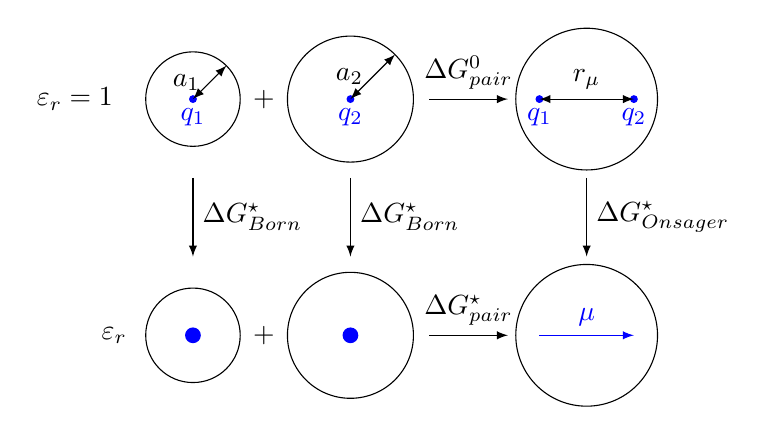
\begin{tikzpicture}
		\draw (-1.5,0) node{$\varepsilon_r=1$};
		\draw (-1,-3) node{$\varepsilon_r$};
		\draw (0,0) circle (.6cm);
		\fill[blue] (0,0) node[below]{$q_1$}  circle (.05cm);
		\draw[latex-latex] (0,0) -- (45:0.6) node[midway,left]{$a_1$};
		
		\draw (.9,0) node{+};
		
		\draw (2,0) circle (.8cm);
		\fill[blue] (2,0) node[below]{$q_2$}  circle (.05cm);
		\draw[latex-latex] (2,0) -- +(45:0.8) node[midway,left]{$a_2$};
		
		\draw[-latex] (3,0) -- +(1,0) node[midway,above]{$\Delta G^0_{pair}$};
		
		\draw (5,0) circle (.9cm);
		\fill[blue] (4.4,0) node[below]{$q_1$} circle (.05cm);
		\fill[blue] (5.6,0) node[below]{$q_2$}  circle (.05cm);
		\draw[latex-latex](4.4,0) -- (5.6,0) node[midway,above]{$r_\mu$};
		
		\draw[-latex] (0,-1) -- +(0,-1) node[midway,right]{$\Delta G^\star_{Born}$};
		\draw[-latex] (2,-1) -- +(0,-1) node[midway,right]{$\Delta G^\star_{Born}$};
		\draw[-latex] (5,-1) -- +(0,-1) node[midway,right]{$\Delta G^\star_{Onsager}$};
		
		\fill[blue] (0,-3) circle (.1cm);
		\draw (0,-3) circle (.6cm);
		
		\draw (.9,-3) node{+};
		
		\draw (2,-3) circle (.8cm);
		\fill[blue] (2,-3) circle (.1cm);	
		
		\draw[-latex] (3,-3) -- +(1,0) node[midway,above]{$\Delta G^\star_{pair}$};
		
		\draw (5,-3) circle (.9cm);
		\draw[-latex,blue](4.4,-3) -- (5.6,-3) node[midway,above]{$\mu$};
	\end{tikzpicture}
	\caption{Thermodynamic cycle for the formation of ion-pair, adapted from Ref.~\citenum{lundDielectricInterpretationSpecificity2010}.}
	\label{fig:ionpair}
\end{figure}

This qualitative model (see Fig.~S3) indicates that ion pairing depends on: \begin{inparaenum}[(i)]
	\item the ratio $\chi = a_1 / a_2$, with $\chi \sim 1$ leading to the lowest pair formation energy (as previously noted by Lund and colleagues),
	\item the attraction between the charges ($s_1$),
	\item the shape of the final cavity (pairing energy increases with $s_2$), and
	\item the dielectric constant $\varepsilon_r$.
\end{inparaenum}
While the latter parameter has only a minor influence (although the difference increases with $s_1$), the formation of a pair of ions is favored in less polar solvents, as expected.

It is worth noting that the impact of the ratio between the radii of different species has been observed by other researchers. For instance, Wylie and co-workers reported in Ref.~\citenum{wylieIncreasedStabilityNitroxide2019b} that the stabilization of the cation-radical pair, \ce{N^.C+}, by the anion is inversely proportional to the size of the latter. However, it should also be noted that the Debye-Hückel (DH) correction presented above tends to favor individual ions (which are more stabilized at high $[X]$ due to the increase of $\kappa$) rather than large, and generally neutral, complexes.


\subsection{Counterion as a fictitious particle}

Alternatively, Matsui et al. \cite{matsuiDensityFunctionalTheory2013} proposed that the impact of counterions on the redox potential of $X^z$ could be described using a single fictitious particle, $P^{-z}$, with a radius $a=fa_0$ proportional to that of the redox species, $a_0$ (considered constant for all oxidation states of $X$), and bearing the appropriate counter-charge, $-q$. They suggested evaluating the energy of this particle using a modified Born approach [Eq.~\eqref{eq:born}]:\begin{align}
	&\Delta G^\star_{Mat}(P^z) = \frac{1}{4\pi\epsilon_0}\, \frac{q^2}{2fa_0}\,\left[\frac{1}{\varepsilon_r}-1\right]\,\erf(\mu\,a_0\,|q|),
\end{align}
where $f$ and $\mu$ are method-dependent factors, the latter being described in Ref.~\citenum{matsuiDensityFunctionalTheory2013} as a parameter to induce a screening effect near the redox center.


In the presence of this fictitious particle, the reduction of $X^z$ becomes:\begin{equation*}
	\begin{array}{rl}
		X^z + n_e\,e^- &\rightarrow X^{z-n_e} \\
		P^{-z} \phantom{ + n_e\,e^-} &\rightarrow P^{n_e-z} + n_e\,e^- \\
		\hline
		X^z + P^{-z}&\rightarrow X^{z-n_e} +P^{n_e-z}\\
	\end{array}  \label{eq:corr}
\end{equation*}
and therefore,\begin{align}
	E^{Mat}_{abs}(X^z|X^{z-n_e}) &= 	E_{abs}^0(X^{z}|X^{z-n_e}) -\frac{1}{n_e\,F}\,[\Delta G^\star_{Mat}(P^{n_e-z}) - \Delta G^\star_{Mat}(P^{-z})] \nonumber\\
	&= 	E_{abs}^0(X^{z}|X^{z-n_e}) -\frac{\Delta\Delta G^\star_P}{n_e\,F}, \label{eq:matsui} 
\end{align}
where:\begin{align*}
	\Delta\Delta G^\star_{Mat}&=\frac{1}{4\pi\epsilon_0}\frac{1}{2fa_0}\,\left[\frac{1}{\varepsilon_r}-1\right]\times\nonumber\\
	&\left[ (n_e-q)^2\,\erf(\mu\,a_0\,|n_e-q|)-q^2\,\erf(\mu\,a_0\,|q|)\right].
\end{align*}
Matsui and co-workers proposed to  find the parameter $f$ and $\mu$ so that they minimize the difference between $E^{Mat}_{rel}(X^z|X^{z-n_e})$  [from Eq.~\eqref{eq:ecalc}] and experimental $E^0_{rel}(X^z|X^{z-n_e})$ values.  Note that therefore they consider that $ E^{0}_{abs}(\text{SHE})$ is a third fitting parameter.

\section{Compounds and computational chemistry aspects} \label{sec:methodo}

In this study, the set of nitroxides considered by Hodgson \textit{et al.} (compounds \textbf{1}-\textbf{54}) is examined, supplemented with a few additional compounds to increase the number of experimental values (\textbf{55}-\textbf{61}). All structures are depicted in Fig.~\ref{fig:nitroxides}. The \ce{AC} pair, consisting of \ce{BF4^-} (\ce{A^-}) and \ce{NMe4^+} (\ce{C^+}), is used as electrolyte. These ions were chosen because they are good models of electrolytes used in the experimental measurements discussed in Section \ref{sec:exp}. While other pairs have been shown to have a larger effect on the redox potential \cite{wylieImprovedPerformanceAllOrganic2019a}, the trends among the families and substituents should remain consistent.

\begin{figure}[!p]
\centering
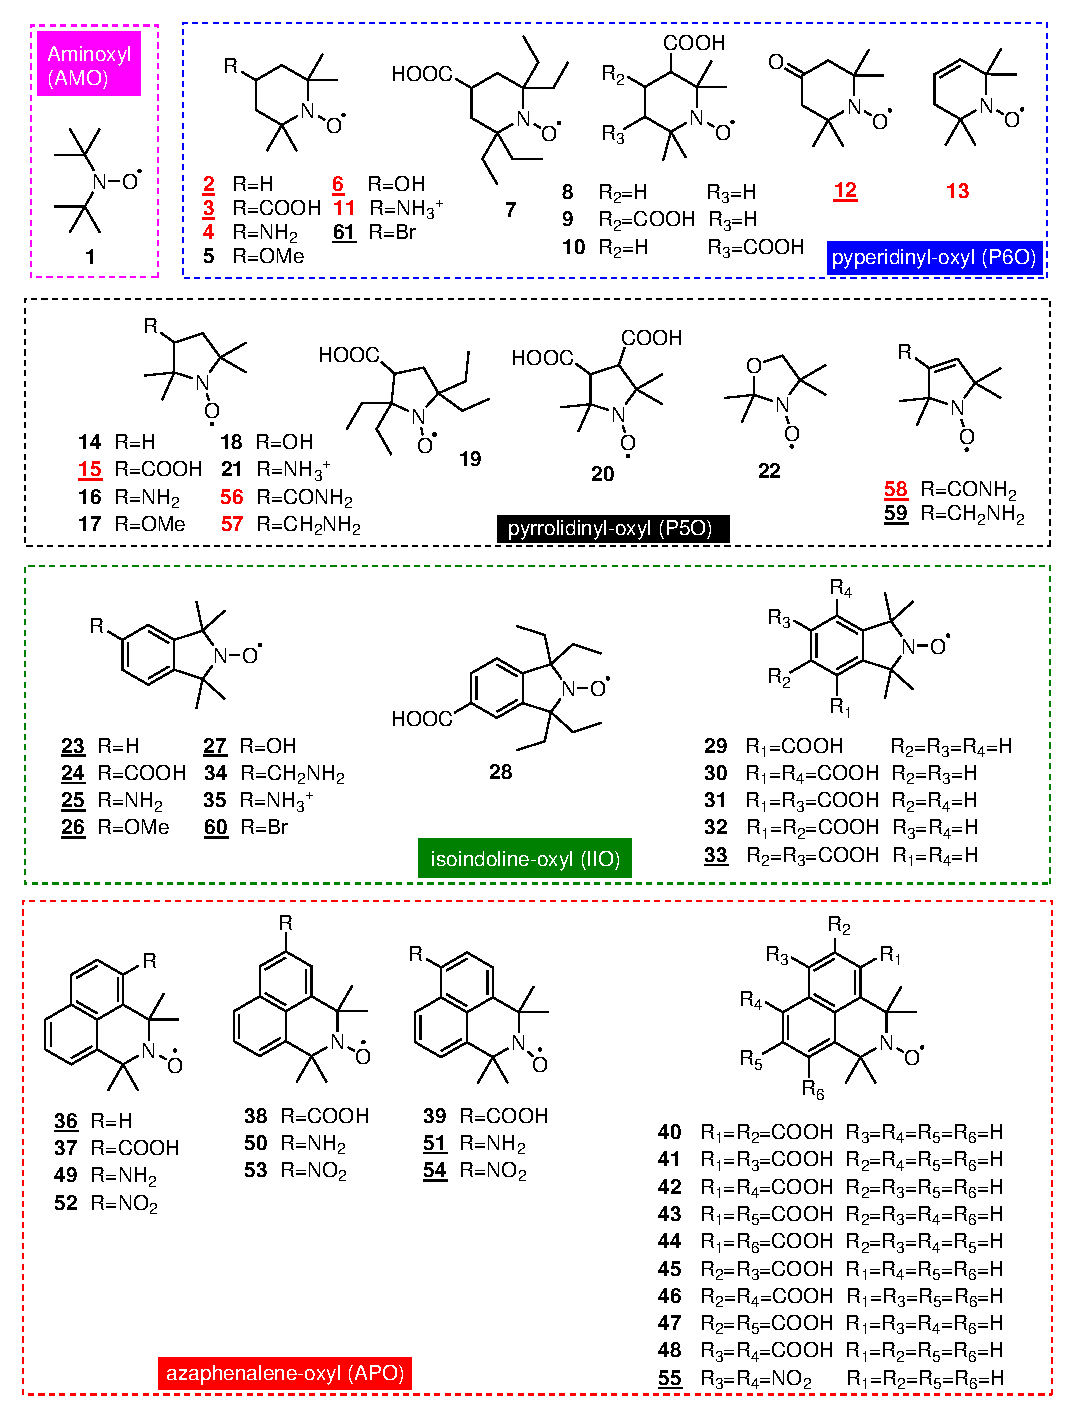
\includegraphics[width=\linewidth]{Figure7}
\caption{Selected nitroxides, sorted by families. Compounds \textbf{1}-\textbf{54} are from Ref.~\citenum{hodgsonOneElectronOxidationReduction2007}.  If the compound number is written in red, experimental (oxidation) potentials are available in water, while in acetonitrile if the number is underlined.}
\label{fig:nitroxides}
\end{figure}

Geometry optimizations and subsequent vibrational frequency calculations were performed at the density functional theory (DFT) level with the $\omega$B97X-D exchange-correlation functional (XCF), with the 6-311+G(d)  basis set. The solvent effects are included using the SMD approach \cite{marenichUniversalSolvationModel2009} approach. All calculations were performed with Gaussian 16 C02 \cite{g16}. With other possible candidates, this XCF have been demonstrated to  provide reliable geometries (see Ref.~\citenum{wylieImprovedPerformanceAllOrganic2019a}) and redox potentials  \cite{flores-leonarFurtherInsightsDFT2017,maierG4AccuracyDFT2020} (see also Fig.~S4).  For compound \textbf{1}-\textbf{54}, the geometries obtained by Hodgson et al.~\cite{hodgsonOneElectronOxidationReduction2007} have been used as a starting point, taking advantage of their extensive conformational search. All radical forms are considered to have a doublet ground state  [$\braket{S^2}=\frac{3}{4}$]. Then, the same calculations were preformed in acetonitrile for the subset of compounds for which experimental redox potentials are available (Fig.~\ref{fig:nitroxides}). The geometries of the complexes (Fig.~\ref{fig:cip}) were then optimized at the same level of approximation, for which different positions of the counterions have been assessed (\textit{vide supra}). Finally, to study the influence of the substituent on the redox potential with the model presented in Section \ref{sec:eleczhang}, single point calculation are performed at the $\omega$B97X-D/6-311+G(d) level in gas phase, using the optimized geometries of  the radical states of each nitroxides (in water) in which the  $>$\ce{N-O^.} moiety is substituted by \ce{CH_2} (the rest of the geometry is kept fixed).

Since all thermochemical quantities are $\kappa$-dependent, analyses were performed using custom Python scripts. When required (e.g., in Eq.~\eqref{eq:dh}), the value of $a$ (the radius of the solute cavity) is taken as half the largest distance between any pair of two atoms in the molecule. Although this is an approximation, it provides a consistent method to treat all molecules proportionally to their size and it is consistent with other publications \cite{matsuiDensityFunctionalTheory2013}.  Furthermore, a value of $\varepsilon_{r,water}=80$ for water and $\varepsilon_{r,acetonitrile}=35$ for acetonitrile is used. These relative permittivities correspond to those of the pure solvents and are known to be lower for the respective electrolyte solutions \cite{silvaTrueHuckelEquation2022}. These variations can be substantial; for example, $\varepsilon_r \approx 70$ for a solution containing \SI{1}{\mol\per\kilo\gram} of \ce{NaCl} in water \cite{kontogeorgisDebyeHuckelTheoryIts2018, silvaTrueHuckelEquation2022}, but they depend on the nature of the electrolyte, so it was not considered here.


Unless otherwise mentioned, the value of $\kappa^2$ is obtained assuming  $c_{ox} = c_{rad} = c_ {red} = \SI{e-3}{\mole\per\liter}$, a prototypical concentration in measurements.


\section{Results and discussion} \label{sec:results}

\subsection{Structure-activity relationships} \label{sec:sar}

Oxidation and reduction potentials of the nitroxide radicals in water, grouped by family, are plotted in Fig.~\ref{fig:family} (see also Table S1). In comparison to the most simple compound, \textbf{1}, modifying the molecular structure and/or adding substituents generally increases both the oxidation and reduction potentials. Regarding structural impacts, six-membered ring compounds (P6O and APO) exhibit higher reduction potentials than their five-membered ring counterparts (P5O and IIO). Additionally, the incorporation of one or two aromatic rings (IIO and APO) enhances both the oxidation and reduction potentials.


\begin{figure}[!h]
	\centering
	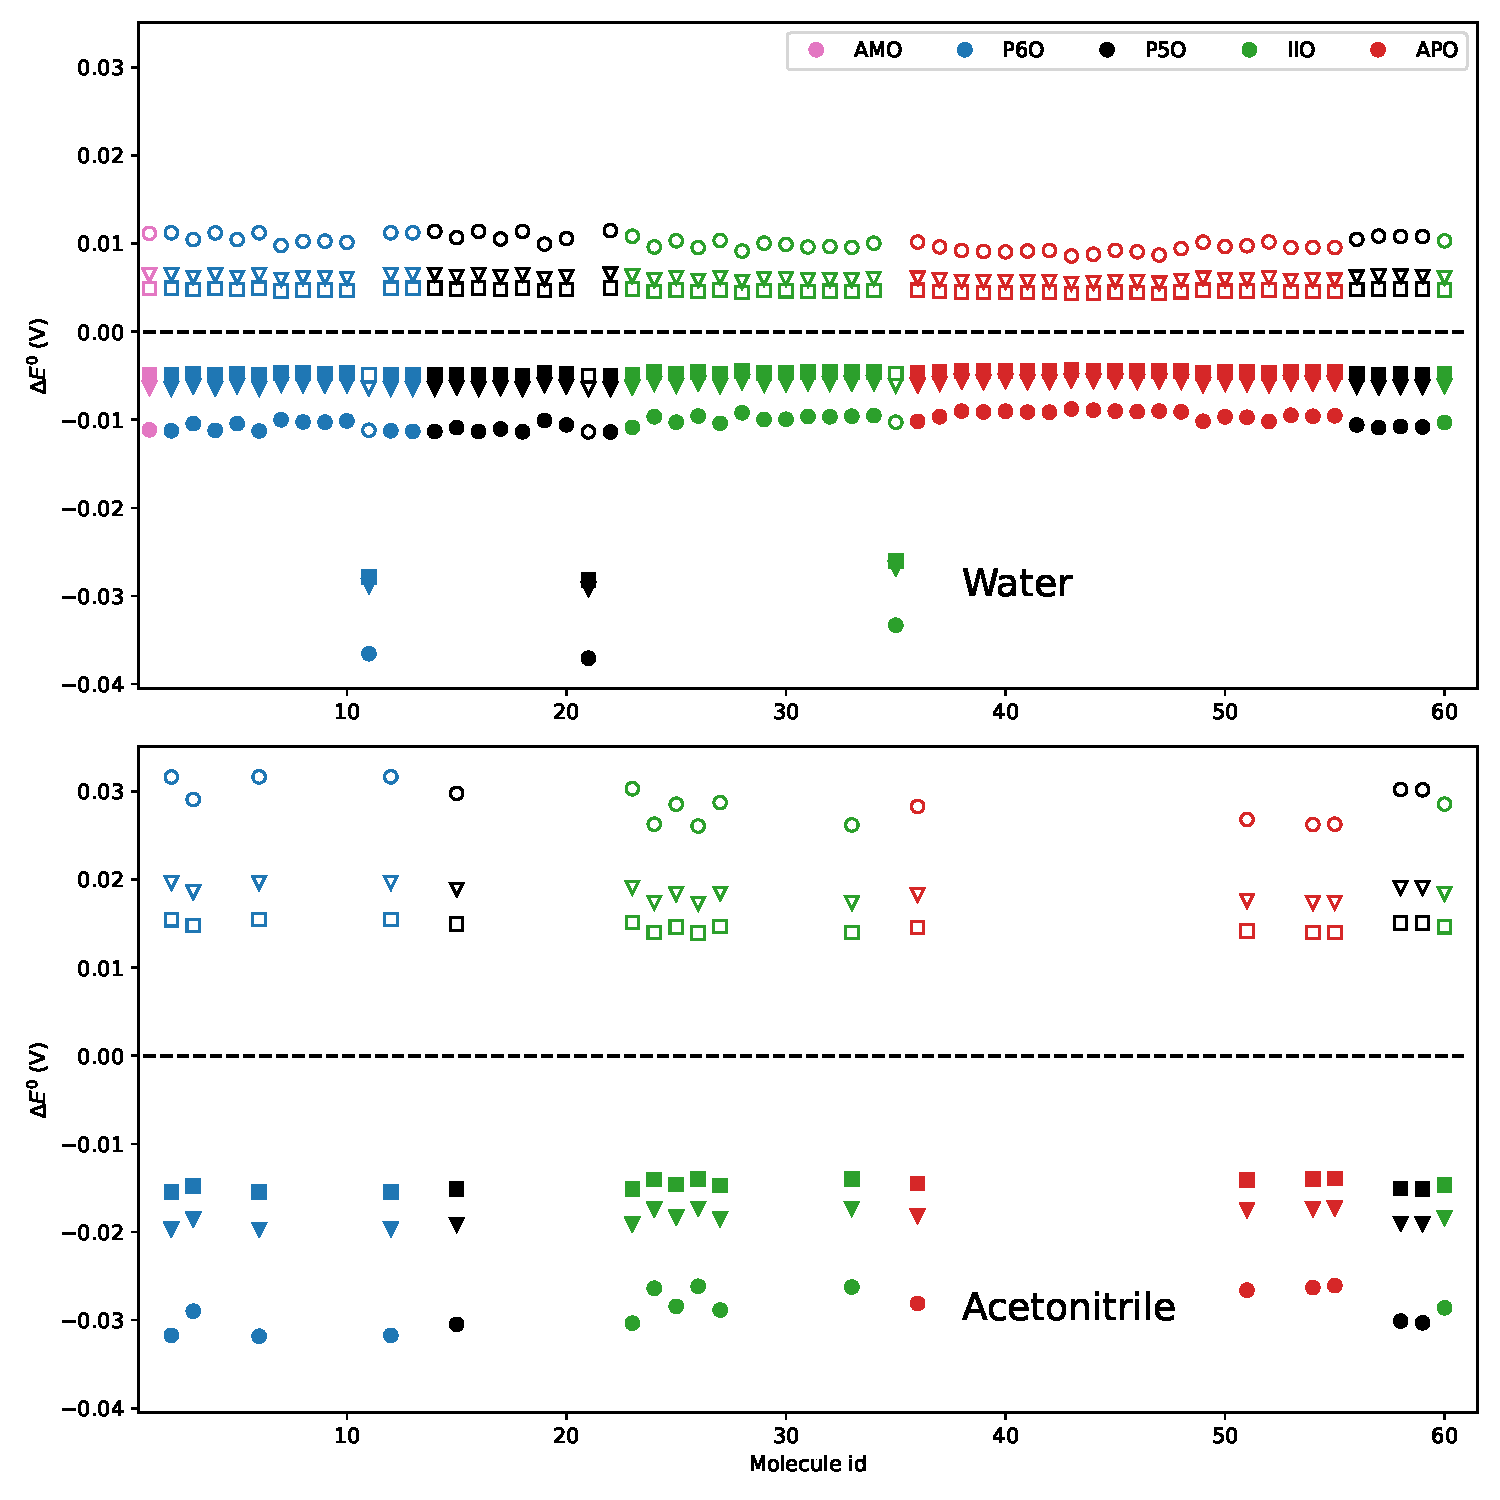
\includegraphics[width=.9\linewidth]{Figure8}
	\caption{Relationship between the absolute oxidation and reduction potentials of nitroxides, as computed at the $\omega$B97X-D/6-311+G(d) level in water (SMD), with a concentration in electrolyte, $[\ce{X}]=\SI{0}{\mole\per\liter}$. The color indicates the family (Fig.~\ref{fig:families}). For each of them, an ellipse is drawn, centered on the mean potential value among the family, whom width and height are given by the standard deviations.}
	\label{fig:family}
\end{figure}

Regarding the impact of substituents, it is noteworthy that non-substituted nitroxides within each family (\textit{i.e.}, \textbf{2}, \textbf{14}, \textbf{23}, and \textbf{36}) have generally one of the lowest oxidation and reduction potentials within their respective groups. Several trends emerge based on the nature of the substituent: \begin{inparaenum}[(i)]
	\item shielding the radical center with ethyl groups instead of methyl groups (\textbf{7}, \textbf{19}, and \textbf{28}) results in a decrease in potentials (particularly the reduction potential), likely due to changes in inductive effects,
	\item protonation of \ce{NH2} (\textit{i.e.}, \textbf{4} vs \textbf{11}, \textbf{16} vs \textbf{21}, and \textbf{25} vs \textbf{35}) increases the potentials, especially in P5O,
	\item multiple substitutions by COOH (\textit{e.g.}, \textbf{8} vs. \textbf{9} and \textbf{10}) also increase the potentials, though the effect is less pronounced in IIO (\textbf{30}-\textbf{33}) and APO (\textbf{41}-\textbf{48}),
	\item consistently with the model described in Section \ref{sec:eleczhang}, compounds with mesomeric donor substituents (\ce{NH2}, \ce{OH}, \ce{OMe}) have lower potentials than those with acceptor substituents (COOH, \ce{NO2}), particularly in aromatic systems (\textit{e.g.}, \textbf{49} vs \textbf{52}), and
	\item compounds \textbf{56} and \textbf{58} have surprisingly low reduction potentials.
\end{inparaenum}
As a consequence, \textbf{55} exhibits the highest oxidation and reduction potentials among all the compounds studied in this paper.

To elucidate these effects, attempts are made to correlate both potentials with Hammett constants for P5O and P6O, but the correlations are found to be very weak, especially for reduction (Fig.~S5). 

The electrostatic interaction model [Eq.~\eqref{eq:Er}] provides more insights. Results are presented in Fig.~\ref{fig:corr} (see also Table S4). It should be noted that this model fails to account for the effect of substituting methyl groups with ethyl groups. Moreover, including the disubstituted compounds (e.g., \textbf{9}, \textbf{10}, \textbf{20}, ...) worsens the correlation ($R^2 \sim 0.5$ and 0.3 for oxidation and reduction, respectively). Compounds \textbf{56} and \textbf{58} remain outliers for reduction. Therefore, all three sets of compounds are treated as outliers in the following discussion.
Though the correlation is poorer for reduction than for oxidation (probably because the electron delocalization means nitrogen is not the atom that should be used to define the origin in that case), this model helps explain the general trends. For instance, the increase in oxidation (and reduction) potential for aromatic compounds correlates with an increase in quadrupole moment ($Q_{xx} > \SI{5}{\elementarycharge\bohr\squared}$ for most members of IIO or APO). Additionally, modifications due to donor/acceptor substituents are linked to changes in the dipole moment. For example, aromatic compounds with \ce{NH2} as a substituent (\textit{e.g.}, \textbf{51}) are characterized by $\mu_{x} < 0$, which increases for compounds with \ce{COOH} (\textit{e.g.}, \textbf{39}) or \ce{NO2} (\textit{e.g.}, \textbf{54}). Furthermore, members of P5O generally present a smaller value of $U_r$ than P6O (\textit{e.g.}, \textbf{17} versus \textbf{5}), which correlates with the increase in oxidation potential observed between these two families. The same trend is observed between APO and IIO.
This model also accounts for some effects due to the position of the substituent (see, e.g., \textbf{49}-\textbf{51}), which was not the case with the original model by Zhang and co-workers (resulting in weak correlations, $R^2 \leq 0.3$). 

Finally, although this model is not directly applicable to positively charged substituents (\textbf{11}, \textbf{21}, and \textbf{35}), for which the dipole and higher multipole moments are ill-defined, the only term of Eq.~\eqref{eq:Er}  would be $q'/r$ (where $q'$ is the charge of the substituent), resulting in a positive contribution to $U_q$ (and a destabilizing interaction with \ce{N+} and \ce{N^.}, while stabilizing \ce{N-}, see Fig.~\ref{fig:dipole}), which correlates well with the increase in oxidation and reduction potentials for these compounds.


\begin{figure}[!h]
\centering
\includegraphics[width=\linewidth]{Figure9}
\caption{Relationship between absolute oxidation (top) and reduction (bottom) potentials of nitroxides and the electrostatic potential between the redox center ($>$\ce{N-O^.}) and the substituent, as computed using \eqref{eq:Er} at the $\omega$B97X-D/6-311+G(d) level in water (SMD), in the limit of $[\ce{X}]=\SI{0}{\mole\per\liter}$. Triangular marker ($\blacktriangle$) indicates results that are excluded from the correlation (see text).}
\label{fig:corr} 
\end{figure}

\clearpage

\subsection{Impact of the solvent} \label{sec:solv}

The solvent exerts a significant stabilizing effect on the charge. In the gas phase (Table S2), $E^0_{abs}(\ce{N+}|\ce{N^.})$ values are around \SI{7}{\volt} (and up to \SI{10}{\volt} for \textbf{11}, \textbf{21}, and \textbf{35}), while $E^0_{abs}(\ce{N^.}|\ce{N-})$ values are approximately \SI{0.3}{\volt} (around \SI{3}{\volt} for \textbf{11}, \textbf{21}, and \textbf{35}). The modifications due to the solvent, primarily resulting from the stabilization of the charges (as indicated by the Born model), but also including moderate geometry changes, amount to about \SI{2}{\volt} (\SI{200}{\kilo\joule\per\mole}).

The difference between redox potentials computed in water and acetonitrile is reported in Fig.~\ref{fig:watvsac} (see also Table S3):  the oxidation potential is only minimally affected, while there is a disparity greater than \SI{0.5}{\volt} for the reduction potentials. In first approximation, the Born model [Eq.~\eqref{eq:born}] can, again, account for these findings: for the oxidation, the change in potentials in the two solvents, $E^0_{acetonitrile} - E^0_{water}$, is proportional to $\varepsilon_{r,acetontrile}^{-1}-\varepsilon_{r,water}^{-1}$, which is positive (assuming that \ce{N^.} is neutral, which holds true for the subset of compounds considered here), whereas for the reduction, it is proportional to $\varepsilon_{r,water}^{-1}-\varepsilon_{r,acetonitrile}^{-1}$, which of the same amplitude, but opposite sign. Since this impact is systematic, similar trends (in terms of the impact of substituents) between redox potentials in water and acetonitrile are observed.


\begin{figure}[!h]
	\centering
	\includegraphics[width=.8\linewidth]{Figure10}
	\caption{Comparison between the absolute oxidation (top) and reduction (bottom) potentials of nitroxides as computed at the $\omega$B97X-D/6-311+G(d) level in water and acetonitrile (SMD),  in the limit of $[\ce{X}]=\SI{0}{\mole\per\liter}$. The dashed line represents no change. }
	\label{fig:watvsac}
\end{figure}

\clearpage
\subsection{Impact of the electrolytes} \label{sec:elect}

So far, the concentration of electrolyte, $[X]$, has been maintained at zero. To evaluate its impact on the redox potentials, the DH correction itself, Eq.~\eqref{eq:dh}, is initially examined in Fig.~\ref{fig:DH}. As anticipated due to the amplitude of the charges involved ($z=\pm 1$), it remains small within the concentration range considered here (a few tenths of millivolts for $[X] \leq \SI{1}{\mole\per\liter}$ and larger in acetonitrile), increasing with $[X]$. Its sign differs between oxidation and reduction potentials, since it only affects the charged species, and while \ce{N+} is a reactant, \ce{N-} a product. Additionally, it decrease for compounds belonging to the IIO and APO families (as they are larger molecules with larger $a$), while it is amplified for species with a net positive charge (\textbf{11}, \textbf{21}, \textbf{35}), for which the correction for oxidation and reduction potentials is negative.


\begin{figure}[!b]
	\centering
	\includegraphics[width=\linewidth]{Figure11}
	\caption{Impact of the Debye-Hückel correction, as $\Delta E^0 = -\frac{\Delta \Delta G_{DH}^\star}{F}$ for $[X]=\SI{1}{\mole\per\liter}$ (round markers), $[X]=\SI{0.1}{\mole\per\liter}$ (triangular markers, $\blacktriangle$)  and $[\ce{X}]=\SI{0}{\mole\per\liter}$ (square markers, $\blacksquare$), as computed at the $\omega$B97X-D/6-311+G(d) level in water (top) and acetonitrile (bottom) using SMD. Filled (empty) markers represent the correction to the oxidation (reduction) potential. }
	\label{fig:DH}
\end{figure}

\clearpage

Then, the formation of the ion pairs is addressed. As noted by other researchers \cite{zhangInteractionsImidazoliumBasedIonic2016,wylieImprovedPerformanceAllOrganic2019a}, the position of the ions significantly impacts the complexation energies. In practice, it is observed that there are two possible positions for the counterion (see Tables S5-S6 and an example in Fig.~\ref{fig:pos-anion}):
\begin{inparaenum}[(i)]
	\item near the redox center ($>$\ce{N-O}), "in front" of the methyl groups, and
	\item near the substituent, "behind" the methyl groups.
\end{inparaenum}

\begin{figure}[!h]
\centering
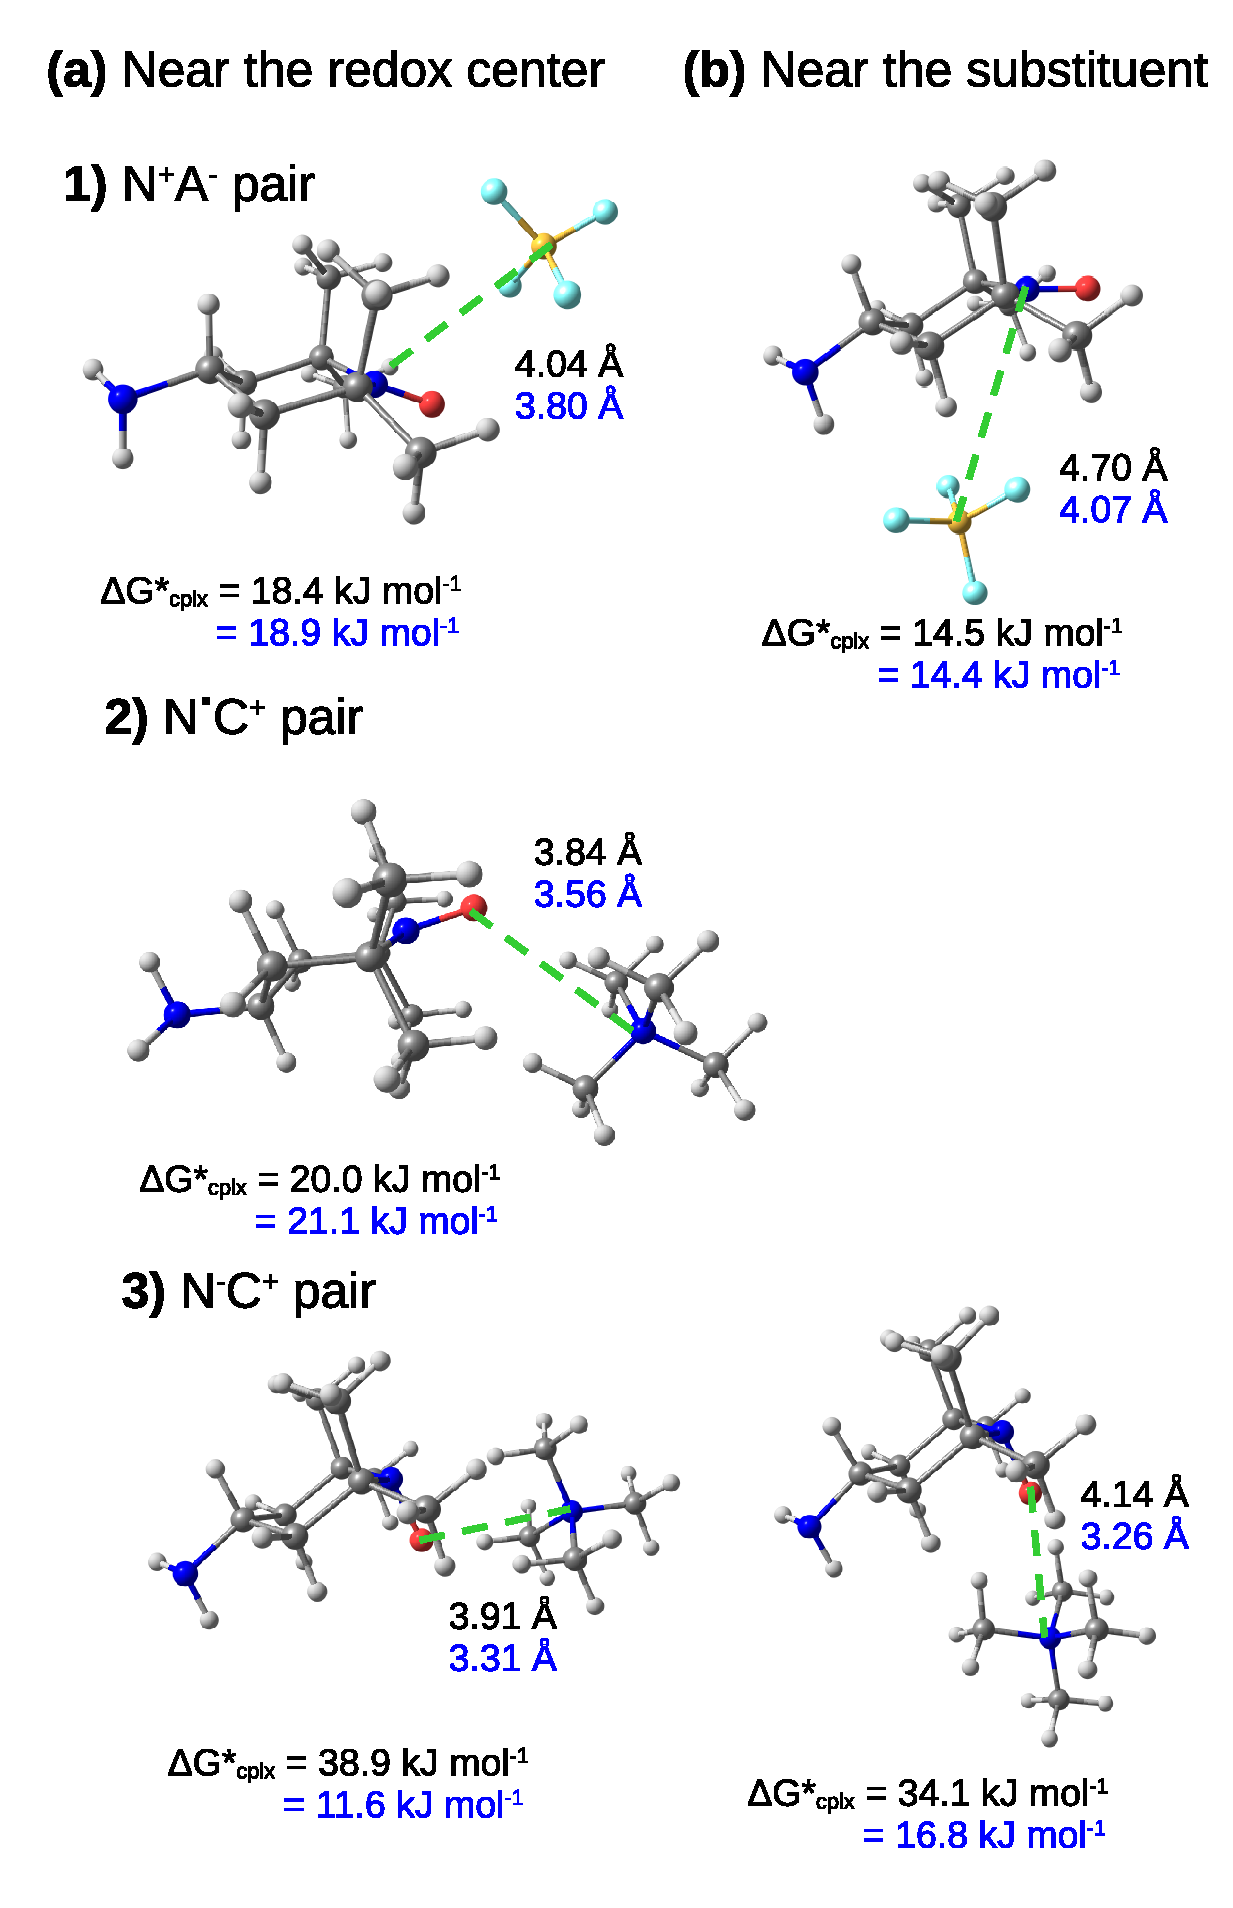
\includegraphics[width=.8\linewidth]{Figure12}
\caption{$\Delta G^\star_{cplx}$ of compound \textbf{4} as a function of counterion poisition. The distance between the redox center (the nitrogen in the oxidized form, $>$\ce{N+=O}, or the oxygen in the reduced form, $>$\ce{N-O-}) and the counterion are also given. Calculations were performed at the $\omega$B97X-D/6-311+G(d) level in water (black) and acetonitrile (blue) using SMD, in the limit of $[X]=\SI{0}{\mole\per\liter}$.}
\label{fig:pos-anion}
\end{figure}

In both solvents, the radical (\ce{N^.}) interacts with \ce{C+} in the first position, near  $>$\ce{N-O^.} \cite{zhangEffectHeteroatomFunctionality2018}. Then, in water, the complexation energies for the \ce{N+A-} and \ce{N^-C+} pairs are positive and significant. The difference in complexation energies between the two positions is generally small (a few \si{\kilo\joule\per\mole}), but the second position is favored in most of the case. Interestingly, this type of interaction corresponds to a larger nitroxide-to-counterion distance, indicating a smaller electrostatic interaction between the redox center and the counterion and suggesting that the substituent also plays a role in lowering the complexation energy. Another contributing factor is the quadrupole-ion interaction due to the aromatic moieties present in compounds from the IIO and APO families, which is particularly important in the \ce{N^-C+} pair. Here, the difference in energy between the two positions is more pronounced.

In acetonitrile, however, the lower dielectric constant leads to a reduced charge screening. A significant decrease of the complexation energy (10 to \SI{20}{\kilo\joule\per\mole}) is observed for the \ce{N^-C+} pair when \ce{C+} is near the nitroxyl group (first position). This aligns with the model for ion pair formation [Eq.~\eqref{eq:pair}], particularly when considering the impact of the ratio between the radii of the cavities. Since \ce{NMe4+} has a larger radius (\SI{2.1}{\angstrom}) than \ce{BF4-} (\SI{1.5}{\angstrom}), the former is closer in size to nitroxides ($>$\SI{3}{\angstrom}). The second position remains generally favored in the \ce{N+A-} pair, though only by a few \si{\kilo\joule\per\mole}.

Using the most stable positions for each complex, the corresponding equilibrium constants are reported in Fig.~\ref{fig:Kx1} (see also Tables S7-S8 and Fig.~S6). The average value in each family, in water, is also reported in Table \ref{tab:Kx1}. In general, $K_{11} < K_{01} < K_{21} < 1$, indicating that the interaction between the hydroxylamine anion and the cation is the less destabilizing. Furthermore, while these equilibrium constants are of the same order of magnitude ($\sim \num{e-5}$) for \textbf{1}, significant differences appear in the other families. 
In particular, in water, the equilibrium constants $K_{01}$ and $K_{21}$ for aromatic compounds, IIO and APO, are two orders of magnitude larger due to ion-quadrupole interactions. The latter family contains compounds with some of the lowest complexation energies. However, correlating the nature of the substituent with the complexation energy remains challenging. In the literature, perpendicular $\pi$-cation interactions are stabilized by electron-rich aromatic rings (and thus donor substituents), while $\pi$-anion interactions are stabilized by electron-poor rings (acceptor substituents) \cite{pappFourFacesInteraction2017}. Despite this, compounds with either donor (\textit{e.g.}, \textbf{42}) or acceptor (\textit{e.g.}, \textbf{54}) substituents exhibit small complexation energies, likely due to variations in ion positioning across different systems. Regarding acetonitrile, while $K_{21}$ increases for the reasons discussed, this is not necessarily the case for the other constants. 

\begin{figure}[!h]
	\centering
	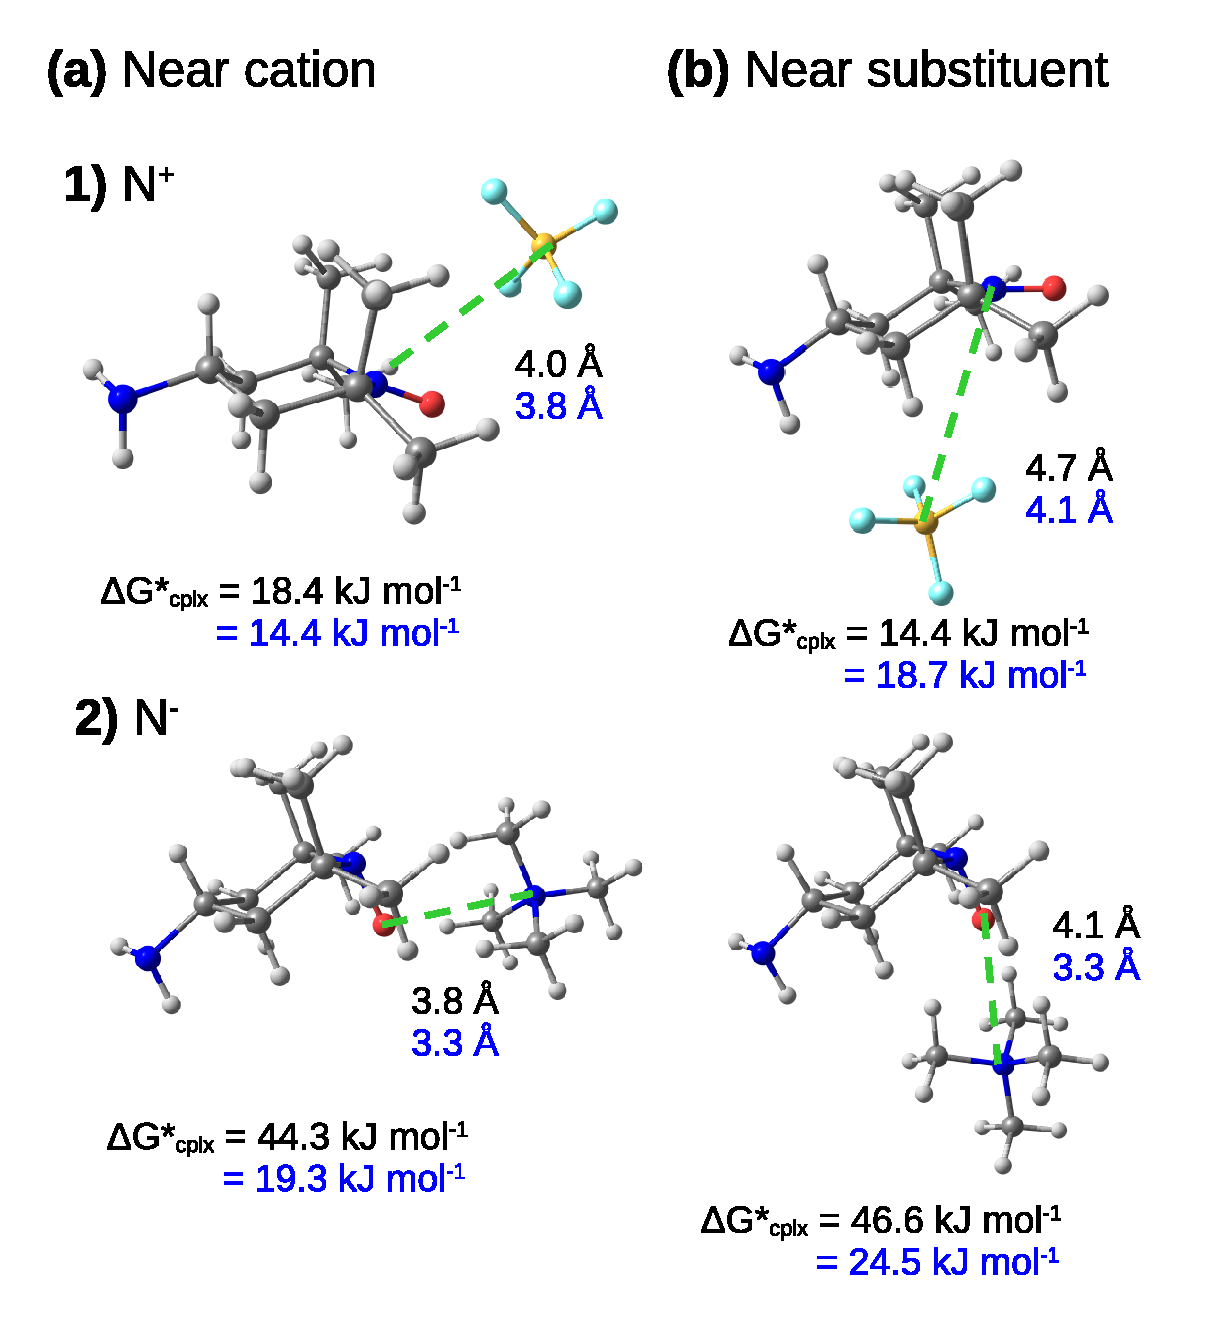
\includegraphics[width=\linewidth]{Figure13}
	\caption{Value of the complexation equilibrium constants $K_{01}$ (triangular markers, $\bullet$), $K_{11}$ (round markers, $\blacktriangle$), and $K_{21}$ (square markers, $\blacksquare$), as computed at the $\omega$B97X-D/6-311+G(d) level in water (top) and acetonitrile (bottom) using SMD and $[X]=\SI{1}{\mole\per\liter}$. The dashed line is for visualization purposes.}
	\label{fig:Kx1}
\end{figure}

\begin{table}[!h]
	\centering
	\begin{tblr}{lccc}
		\hline
		& $\log_{10}K_{01}$ & $\log_{10}K_{11}$ & $\log_{10}K_{21}$ \\
		\hline
		AMO & -4.13 & -4.65 &  -5.15  \\
		P6O & -3.20 $\pm$ 0.70 & -5.54 $\pm$ 0.73 &  -7.52 $\pm$ 1.36 \\
		P5O & -4.38 $\pm$ 1.83 & -5.44 $\pm$ 1.84 &  -3.80 $\pm$ 1.85 \\
		IIO & -3.24 $\pm$ 0.54 & -4.64 $\pm$ 0.40 &  -3.22 $\pm$ 0.81 \\
		APO & -3.22 $\pm$ 0.39 & -5.26 $\pm$ 1.83 &  -2.41 $\pm$ 1.18 \\
		\hline
	\end{tblr}
	\caption{Mean value of the complexation equilibrium constants for each family (reported as mean $\pm$ standard deviation), as computed at the $\omega$B97X-D/6-311+G(d) level in water using SMD and $[X]=\SI{1}{\mole\per\liter}$.}
	\label{tab:Kx1}
\end{table}

A notable exception to these trends is the P6O family, which shows smaller complexation equilibrium constants for the \ce{N^-C+} pair (with $\Delta G^\star_{cplx} > \SI{40}{\kilo\joule\per\mole}$) than others. This is a geometric effect: in such compounds, the \ce{N+=O} group (in oxoammonium) occupies an equatorial position, while the \ce{N-O-} bond (in the hydroxylamine anion) adopts an axial position. Nearby methyl groups hinder electrostatic interactions in the first case, especially for bulky counterions such as \ce{NMe4+}, as seen in Fig.~\ref{fig:pos-anion}. This effect is less pronounced in other families, where the skeleton prevents the oxygen from adopting such a position (particularly in IIO and APO), resulting in larger complexation equilibrium constants when the i ion is in close interaction with the redox center.

Finally, the complexations of the nitroxides to the \ce{AC} pair is considered (Fig.~\ref{fig:Kx2}, Tables S9-S10). Based on the positioning of the ions in the pairs that were previously discussed, for the \ce{N^-AC} and \ce{N^.AC} complexes, the cation is placed near the nitroxyl moiety, while the anion is placed near the substituent. The opposite is done for \ce{N^+AC}. As expected, the equilibrium constants are smaller (by about four orders of magnitude, $\Delta G^\star_{cplx} \sim \SI{50}{\kilo\joule\per\mole}$) than the ones previously discussed. However, the trends are similar: for example, in acetonitrile, the \ce{NAC^-} complexes are more stable than the others, as also observed previously \cite{wylieImprovedPerformanceAllOrganic2019a}. The stabilization of \ce{NAC^.} is however less important in this work than observed by this team, probably because of the larger dielectric constant used here.


\begin{figure}[!h]
\centering
\includegraphics[width=\linewidth]{Figure14}
\caption{Value of the complexation equilibrium constants $K_{02}$ (round markers, $\bullet$), $K_{12}$ (triangular markers, $\blacktriangle$) and $K_{22}$ (square markers, $\blacksquare$) for the 3 oxidation state of nitroxides, as computed at the $\omega$B97X-D/6-311+G(d) level in water (top) and acetonitrile (bottom) using SMD and $[X]=\SI{1}{\mole\per\liter}$.  The dashed line is used to help visualization. }
\label{fig:Kx2}
\end{figure}

\clearpage
\subsection{Comparison to experiment} \label{sec:exp}

A comparison between theoretical (including all corrections discussed above) and experimental oxidation potentials is shown in Fig.~\ref{fig:expvstheo}. Excluding compounds bearing an \ce{NH2} group (so,  \textbf{57} in water, and \textbf{4}, \textbf{51}, and \textbf{59} in acetontrile) results in an excellent linear correlation ($R^2 > 0.9$). Note that the computed potentials for compounds with \ce{NH2} are higher (by more than $\SI{0.1}{\volt}$) than the fit line, suggesting that the amine group might be protonated under the experimental measurement conditions. This is indeed consistent with other cases (\textit{e.g.}, \textbf{25} vs \textbf{35}) discussed in Section \ref{sec:sar}. 

The remaining results indicate that the method used in this paper tends to overestimate the oxidation potentials in water and systematically underestimate them in acetonitrile, with a large mean average error (MAE). This suggests that the value for $E^0_{abs}(\text{SHE})$ might not be appropriate in this solvent. The impact of the different corrections (see Fig.~S7) is to decrease the potential, mainly due to the DH correction (given the value of the complexation equilibrium constants for the oxidation reaction, see Table \ref{tab:Kx1}), as seen in Fig.~\ref{fig:DH}. While this improves the slope and MAE in water, the opposite effect is observed in acetonitrile.

\begin{figure}[!h]
	\centering
	\includegraphics[width=.75\linewidth]{Figure15}
	\caption{Comparison between experimental ($E^0_{rel} $ vs SHE, from Table S11) and  calculated relative oxidation potential ($E^f_{rel}$, computed using \eqref{eq:ef1}, vs SHE) in water (top) and acetonitrile (bottom), as computed at the $\omega$B97X-D/6-311+G(d) level using SMD and $[X]=\SI{0.1}{\mole\per\liter}$.  The dashed line is a linear regression.}
	\label{fig:expvstheo}
\end{figure}

For comparison, the model by Matsui and co-workers \cite{matsuiDensityFunctionalTheory2013} is used in Fig.~\ref{fig:matsui}. The different parameters were determined by fitting the experimental data. It should be noted that for such an oxidation process (\ce{N+ + e- -> N^.}), the $\Delta\Delta G^\star_P$ correction [Eq.~\eqref{eq:matsui}] can only be positive. As a consequence of this limitation, while the corrected $E^0_{abs}(\text{SHE)}$  predicted by this model is slightly larger than the recommended value in water, it is lower in acetonitrile but this value being smaller than in water is not in agreement with experimental data \cite{marenichComputationalElectrochemistryPrediction2014}. Interestingly, this correction is similar to the value of the MAE reported in Fig.~\ref{fig:expvstheo}. Furthermore, while the slope of the linear regression improves in water, it remains the same in acetonitrile. Finally, both $f$ and $\mu$ are smaller than those reported by Matsui and colleagues, though they treated systems bearing larger charges. Therefore, this model is not well-suited for this case.


\begin{figure}[!h]
	\centering
	\includegraphics[width=.75\linewidth]{Figure16}
	\caption{Comparison between experimental ($E^0_{rel} $ vs SHE, from Table S11) and corrected oxidation potential using the scheme of Matsui et al. \cite{matsuiDensityFunctionalTheory2013} [Eq.~\eqref{eq:matsui}, with the parameters $E_{abs}^0(\text{SHE})$, $f$, and $\mu$ obtained by a least-square procedure, on calculated data without the DH correction], as computed at the $\omega$B97X-D/6-311+G(d) level in water (top) and acetonitrile (bottom). The dashed line is a linear regression. }
	\label{fig:matsui}
\end{figure}

\clearpage
\section{Conclusion} \label{sec:conclusion}

In this paper, the impact of different solute-solvent effects on the redox potentials of nitroxides has been assessed, with a particular emphasis on ionic interactions. While the Born model [Eq.~\eqref{eq:born}] shows that the solvent tends to stabilize charges due to changes in the dielectric constant (especially in polar solvents), other, more subtle effects arise from solute-ion interactions caused by the presence of electrolytes. These electrolytes are found in moderate concentrations (\textit{i.e.,} \SI{0.1}{\mole\per\liter}) during the experimental measurement of redox potentials and in higher concentrations (>$\SI{1}{\mole\per\liter}$) in ionic liquids used for batteries.

The impact of electrolytes is twofold:
\begin{inparaenum}[(i)]
	\item at any concentration, the background of charge further stabilizes charged compounds, as described by the Debye-Hückel (DH) model [Eq.~\eqref{eq:dh}], and
	\item at high concentrations, the formation of ion-pairs modifies the redox properties of nitroxides.
\end{inparaenum}
Both effects have been examined: when the charge of the compound and of the electrolyte constituents is moderate, the DH correction is small. However, the formation of pairs depends on the redox state of the nitroxide and the nature of the intermolecular interactions, which goes beyond a simple pair formation model (Fig.~\ref{fig:ionpair}). Two positions are possible for the ion: near the redox center of the nitroxide, and near its substituent, if any. The ion-substituent interaction (in the second position) generally leads to more favorable complexes (especially when the molecule contains aromatic moieties). However, in acetonitrile, the interaction between the reduced form (hydroxylamine anion) and its cation, positioned near the $>$\ce{N-O-} moiety, is the strongest. This seems to be the case in other low-dielectric environments, as noted by others in an even less polar solvent ($\varepsilon_r$ = 25) \cite{wylieImprovedPerformanceAllOrganic2019a}.

In this work, different families of nitroxides have been considered: 5- (P6O, APO) and 6-membered rings (P5O, IIO) containing the nitroxyl moiety, and with (IIO, APO) or without an aromatic system (P5O, P6O) in close vicinity. The impact of such changes, and of substituents, on the redox potentials is largely explained by the electrostatic interaction model (Fig.~\ref{fig:dipole}) developed by Zhang and co-workers \cite{zhangEffectHeteroatomFunctionality2018}: a large quadrupole moment increases both the oxidation and reduction potentials of nitroxides, while increasing the size of the ring (and thus the distance between the substituent and the nitroxyl) mostly affects the reduction potential. Furthermore, acceptor substituents (such as \ce{NO2}) further increase both potentials. While the impact remains moderate (+\SI{0.4}{\volt}), it is hoped that this will provide design rules for future investigations. It was, however, not possible to correlate the impact of the substitution on the formation of ion-pairs, but it was noticed that the favorable interaction between \ce{N-} and \ce{C+} mentioned was systematically hampered by the nitroxyl in an axial position in P6O. This is another important design rule for future applications.

Finally, a comparison with experiment has been performed. It results in an excellent correlation, but the impact of the corrections presented above is minimal in the solvents considered here (water and acetonitrile) and with the concentrations of electrolytes used experimentally. It would be interesting to compare redox potentials measured under different conditions (such as in ionic liquids). Another factor that should be investigated is the temperature, which would affect both the DH correction (through $\kappa$, Eq.~\eqref{eq:kappa2}) and the complexation equilibrium constant. For example, conventional lithium-ion batteries can operate up to \SI{60}{\degreeCelsius} \cite{maTemperatureEffectThermal2018}, but ionic liquids are stable over extended temperature ranges.
	
\section*{Notes}
The author declare no competing financial interest.

\section*{Acknowledgements}
P.B. thanks Prof. B. Champagne for fruitful discussions, and is grateful to the Excellence of Science (EOS) programme  ECOBAT (EOS No. 40007515) for funding this research. 
The calculations were performed on: \begin{inparaenum}[(i)]
	\item the computers of the Consortium des \'{E}quipements de Calcul Intensif (C\'{E}CI, \url{http://www.ceci-hpc.be}) and particularly those of the Technological Platform of High-Performance Computing, for which the author gratefully acknowledge the financial support of the F.R.S-FNRS, of the Walloon Region, and of the University of Namur (Conventions No. 2.5020.11, U.G006.15, U.G018.19, U.G011.22, 1610468, and RW/GEQ2016), and
	\item on Lucia, the Tier-1 supercomputer of the Walloon Region, infrastructure funded by the Walloon Region (grant agreement No. 1910247).
\end{inparaenum} 
	
	
\bibliographystyle{elsarticle-num-names} 
\bibliography{biblio}
	
\end{document}
\endinput
%%
%% End of file `elsarticle-template-num.tex'.
